\documentclass[12pt, twoside]{article}
\usepackage[letterpaper, margin=1in, headsep=0.5in]{geometry}
\usepackage[english]{babel}
\usepackage[utf8]{inputenc}
\usepackage{amsmath}
\usepackage{amsfonts}
\usepackage{amssymb}
\usepackage{tikz}

\usepackage{pgfplots}
\pgfplotsset{width=9cm,compat=1.9}

\usepackage{venndiagram}

\usepackage{graphicx}
\usepackage{enumitem}
\usepackage{multicol}

\usepackage{fancyhdr}
\pagestyle{fancy}
\fancyhf{}
\renewcommand{\headrulewidth}{0pt} % disable the underline of the header

\fancyhead[LE]{\thepage}
\fancyhead[RO]{\thepage \\ Name: \hspace{4cm} \,\\}
\fancyhead[LO]{BECA / Dr. Huson / IB Mathematics\\* Unit 6: Differential Calculus\\* 11 March 2020}

\begin{document}
\begin{enumerate}
    \subsubsection*{6.10 Do Now : Tangents, systems of equations, use of sine function \\ Calculator practice H}

    \item The reciprocal function $\displaystyle f(x)= \frac{1}{x}+x$ is shown on the axes below.
    \begin{center}
    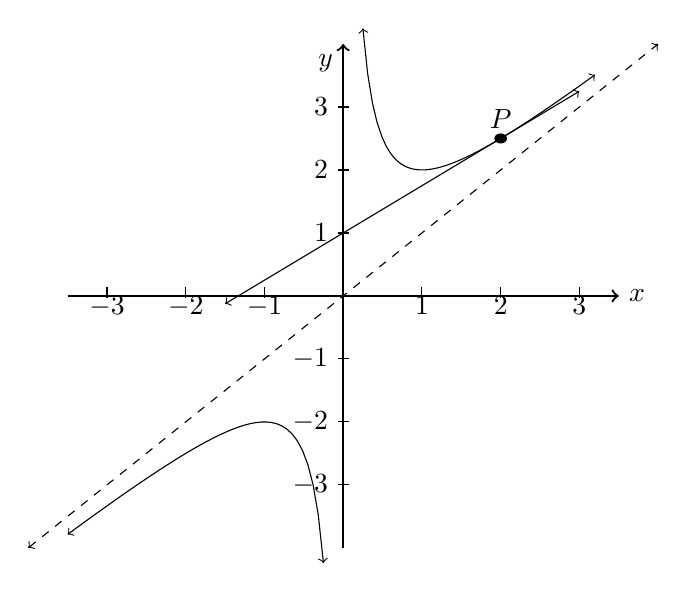
\begin{tikzpicture}[xscale=1.0, yscale=0.8]
        \foreach \x in {-3,-2,-1,1,2,3}
          \draw[shift={(\x,0)},color=black] (0pt,-1pt) -- (0pt,4pt) node[below]  {$\x$};
        \foreach \y in {-3,-2,-1,1,2,3}
          \draw[shift={(0,\y)},color=black] (2pt,0pt) -- (-2pt,0pt) node[left]  {$\y$};
          \draw [thick, ->] (-3.5,0) -- (+3.5,0) node [right] {$x$};
          \draw [thick, ->] (0,-4) -- (0,4) node [below left] {$y$};
        %\fill (1,-4.5) circle[radius=2pt] node [below] {$P$};
        %\fill (0,-4) circle[radius=2pt] node [right] {$Q$};
        \draw [<->] plot[samples=50,domain= 0.25:3.2] (\x, {(1/\x +\x)});
        \draw [<->] plot[samples=50,domain= -3.5:-0.25] (\x, {(1/\x +\x)});
        \draw [<->, dashed] plot[domain= -4:4] (\x, {\x});
        \draw [<->] plot[domain= -1.5:3] (\x, {3/4*\x+1});
        \fill (2,2.5) circle[radius=0.08cm] node[above]{$P$};
    \end{tikzpicture}
    \end{center}
    A tangent to the function at $x=2$ is drawn with the point of tangency $P$.
    \begin{enumerate}%[itemsep=0.8cm]
      \item Write down the derivative of $f$, $f'(x)$. (hint: use a negative exponent) \hfill [2]
      \item Show that the gradient of the tangent line is $\frac{3}{4}$. \hfill [1]
      \item Find the equation of the tangent line. \hfill [2]
      \item Show that there is a local minimum at $x=1$. (hint: show the derivative is zero at $x=1$. Sketch where the function is decreasing then increasing.) \hfill [2]
    \end{enumerate}
    \begin{tikzpicture}
      \draw (0,0) rectangle (15.2,7);
      \draw (8,0) rectangle (15.2,5.5);
      \node at (0,7)[below right]{\textbf{Working:}};
      \node at (8,5.5)[below right]{\textbf{Answers:}};
      \draw [dotted] (9,4.1)node[left]{(a)}--(15,4.1);
      \draw [dotted] (9,3.2)node[left]{(c)}--(15,3.2);
      \draw [dotted] (9,2.3)node[left]{(d)}--(15,2.3);
      \draw [dotted] (9.35,1.4)node[left]{(e)(i)}--(15,1.4);
      \draw [dotted] (9.3,0.5)node[left]{(ii)}--(15,0.5);
  \end{tikzpicture}

  \newpage
    \item The function $f(x)=x\sin x$ is tangent to the line $y=x$ once in each period. Find the coordinates of the first two points of tangency, i.e. for $x >0$.\\[0.25cm] 
    Sketch the graph to show working. \\(note: when a degree measure is used in a function, assume it is in radians.)

        \begin{tikzpicture}
            \draw (0,0) rectangle (15.2,6);
            \draw (8,0) rectangle (15.2,3);
            \node at (0,6)[below right]{\textbf{Working:}};
            \node at (8,3)[below right]{\textbf{Answers:}};
            \draw [dotted] (9,1.7)node[left]{(a)}--(15,1.7);
            \draw [dotted] (9,0.7)node[left]{(b)}--(15,0.7);
        \end{tikzpicture}

\item Given a triangle $\triangle ABC$ with $a=11.3$, $b=15.6$, $\hat{C} = 58^\circ$. 
    \begin{enumerate}
        \item Find the third side length, $c$. \hfill [3]
        \item Find the area of the triangle $\triangle ABC$. \hfill [3]
    \end{enumerate}
        \begin{tikzpicture}
            \draw (0,0) rectangle (15.2,9);
            \draw (8,0) rectangle (15.2,3);
            \node at (0,9)[below right]{\textbf{Working:}};
            \node at (8,3)[below right]{\textbf{Answers:}};
            \draw [dotted] (9,1.7)node[left]{(a)}--(15,1.7);
            \draw [dotted] (9,1)node[left]{(b)}--(15,1);
        \end{tikzpicture}


\end{enumerate}
\end{document}